%!TEX TS-program = xelatex

\documentclass[t]{beamer}  % [t], [c], или [b] --- вертикальное выравнивание на слайдах (верх, центр, низ)
%\documentclass[t, handout]{beamer} % Раздаточный материал (на слайдах всё сразу)
%\documentclass[aspectratio=169, t]{beamer} % Соотношение сторон

\usepackage{epstopdf}

%\usetheme{Berkeley} % Тема оформления
%\usetheme{Bergen}
%\usetheme{Szeged}

%\usecolortheme{beaver} % Цветовая схема
%\useinnertheme{circles}
%\useinnertheme{rectangles}

\usepackage{HSE-theme/beamerthemeHSE} % Подгружаем тему


%%% Работа с русским языком
\usepackage{cmap}					% поиск в PDF
\usepackage{mathtext} 				% русские буквы в формулах
\usepackage[T2A]{fontenc}			% кодировка
\usepackage[utf8]{inputenc}			% кодировка исходного текста
%%% Работа с русским языком и шрифтами
\usepackage[english]{babel}   % загружает пакет многоязыковой вёрстки


%%% Дополнительная работа с математикой
\usepackage{amsmath,amsfonts,amssymb,amsthm,mathtools} % AMS
\usepackage{icomma} % "Умная" запятая: $0,2$ --- число, $0, 2$ --- перечисление

%% Номера формул
%\mathtoolsset{showonlyrefs=true} % Показывать номера только у тех формул, на которые есть \eqref{} в тексте.
%\usepackage{leqno} % Нумерация формул слева

%% Свои команды
\DeclareMathOperator{\sgn}{\mathop{sgn}}

%% Перенос знаков в формулах (по Львовскому)
\newcommand*{\hm}[1]{#1\nobreak\discretionary{}
	{\hbox{$\mathsurround=0pt #1$}}{}}

%%% Работа с картинками
\usepackage{graphicx}  % Для вставки рисунков
\graphicspath{{images/}{images2/}}  % папки с картинками
\setlength\fboxsep{3pt} % Отступ рамки \fbox{} от рисунка
\setlength\fboxrule{1pt} % Толщина линий рамки \fbox{}
\usepackage{wrapfig} % Обтекание рисунков текстом
\usepackage{caption}


%%% Работа с таблицами
\usepackage{array,tabularx,tabulary,booktabs} % Дополнительная работа с таблицами
\usepackage{longtable}  % Длинные таблицы
\usepackage{multirow} % Слияние строк в таблице

%%% Программирование
\usepackage{etoolbox} % логические операторы

%%% Другие пакеты
\usepackage{lastpage} % Узнать, сколько всего страниц в документе.
\usepackage{soul} % Модификаторы начертания
\usepackage{csquotes} % Еще инструменты для ссылок
%\usepackage[style=authoryear,maxcitenames=2,backend=biber,sorting=nty]{biblatex}
\usepackage{multicol} % Несколько колонок

%%% Картинки
\usepackage{tikz} % Работа с графикой
\usepackage{pgfplots}
\usepackage{pgfplotstable}
\usepackage{verbatim}
\usetikzlibrary{fadings}
\usepackage[outline]{contour}
\usepackage{pifont} 

\usepackage{chngcntr} % нумерация графиков и таблиц по секциям
\counterwithin{table}{section}
\counterwithin{figure}{section}

\usepackage{listings}

\lstdefinelanguage{Rust}{
  sensitive=true,
  morekeywords=[1]{
    break, continue, else, for, if, loop, match, return, while, struct
  },
  morekeywords=[2]{
    crate, fn, async, mod, pub, use, self, Self, struct, enum, const, static, let, mut, ref, type, impl, trait, where, as, dyn, move,
  },
  morekeywords=[3]{
    bool, char, i8, i16, i32, i64, isize, u8, u16, u32, u64, usize, f32, f64, str, String,
  },
  morekeywords=[4]{
    Ok, Err, Some, None,
  },
  morekeywords=[5]{
    await,
  },
  keywordstyle=[5]{\color{purple}},
  morecomment=[s]{/*}{*/},
  morecomment=[l]//,
  morestring=[b]",
  morestring=[b]r",
  morestring=[b]'',
}

\lstset{
  language=Rust,
  basicstyle=\ttfamily,
  keywordstyle=\color{blue},
  stringstyle=\color{red},
  commentstyle=\color{green},
  showstringspaces=false,
  breaklines=true,
  frame=none,
}


\lstnewenvironment{rustcode}[1][]{
  \lstset{
    language=Rust,
    basicstyle=\ttfamily,
    keywordstyle=\color{blue},
    stringstyle=\color{red},
    commentstyle=\color{gray},
    showstringspaces=false,
    breaklines=true,
    % frame=single,
    #1
  }
}{}


\lstnewenvironment{cppcode}[1][]{
  \lstset{
    language=C++,
    basicstyle=\ttfamily,
    keywordstyle=\color{blue},
    stringstyle=\color{red},
    commentstyle=\color{gray},
    showstringspaces=false,
    breaklines=true,
    % frame=single,
    #1
  }
}{}

\usepackage{setspace}
\usepackage{color}



\title{Development of Compute Cluster Simulator}
\author[Artem Makogon]{\footnotesize Author: Artem Makogon \\[5pt]   Supervisor: Oleg Sukhoroslov}
\date{\today}
% \institute[Высшая школа экономики]{National Research University\\ 
	% <<Higher School of Economics>>}



\begin{document}
	
	\begin{frame}
		\maketitle
	\end{frame}
	
    \section{Introduction}
    \subsection{Testing of cluster scheduling algorithms}

	\begin{frame}[fragile]
		\frametitle{\insertsection} 
		\framesubtitle{\insertsubsection}
				\vspace{0.5cm}
				\begin{itemize}
					\item Compute clusters are widely used for complex calculations.
					\item Scheduling algorithms are crucial for their performance.
					\item These algorithms are the subject of active research.
				\end{itemize}
				\alt<2->{
					{ \hspace{5cm} \large $\Downarrow$ } 
					\begin{itemize}
						\item[\small\textgreater] Researches need a tool for testing their hypotheses.
						\item[\small\textgreater] Using real clusters is expensive and time-consuming.
					\end{itemize}
				}{}
				\alt<3->{
					{ \hspace{5cm} \large $\Downarrow$ } 
					\begin{itemize}
						\item[\small\ding{51}] \textbf{Simulators} are used for effective development.
					\end{itemize}
				}{}
		
	\end{frame}
	
	\subsection{Cluster architecture}

	\begin{frame}[fragile]
    \frametitle{\insertsection} 
	\framesubtitle{\insertsubsection}
	\vspace{0.1cm}	
	\begin{figure}[H]
		\centering
			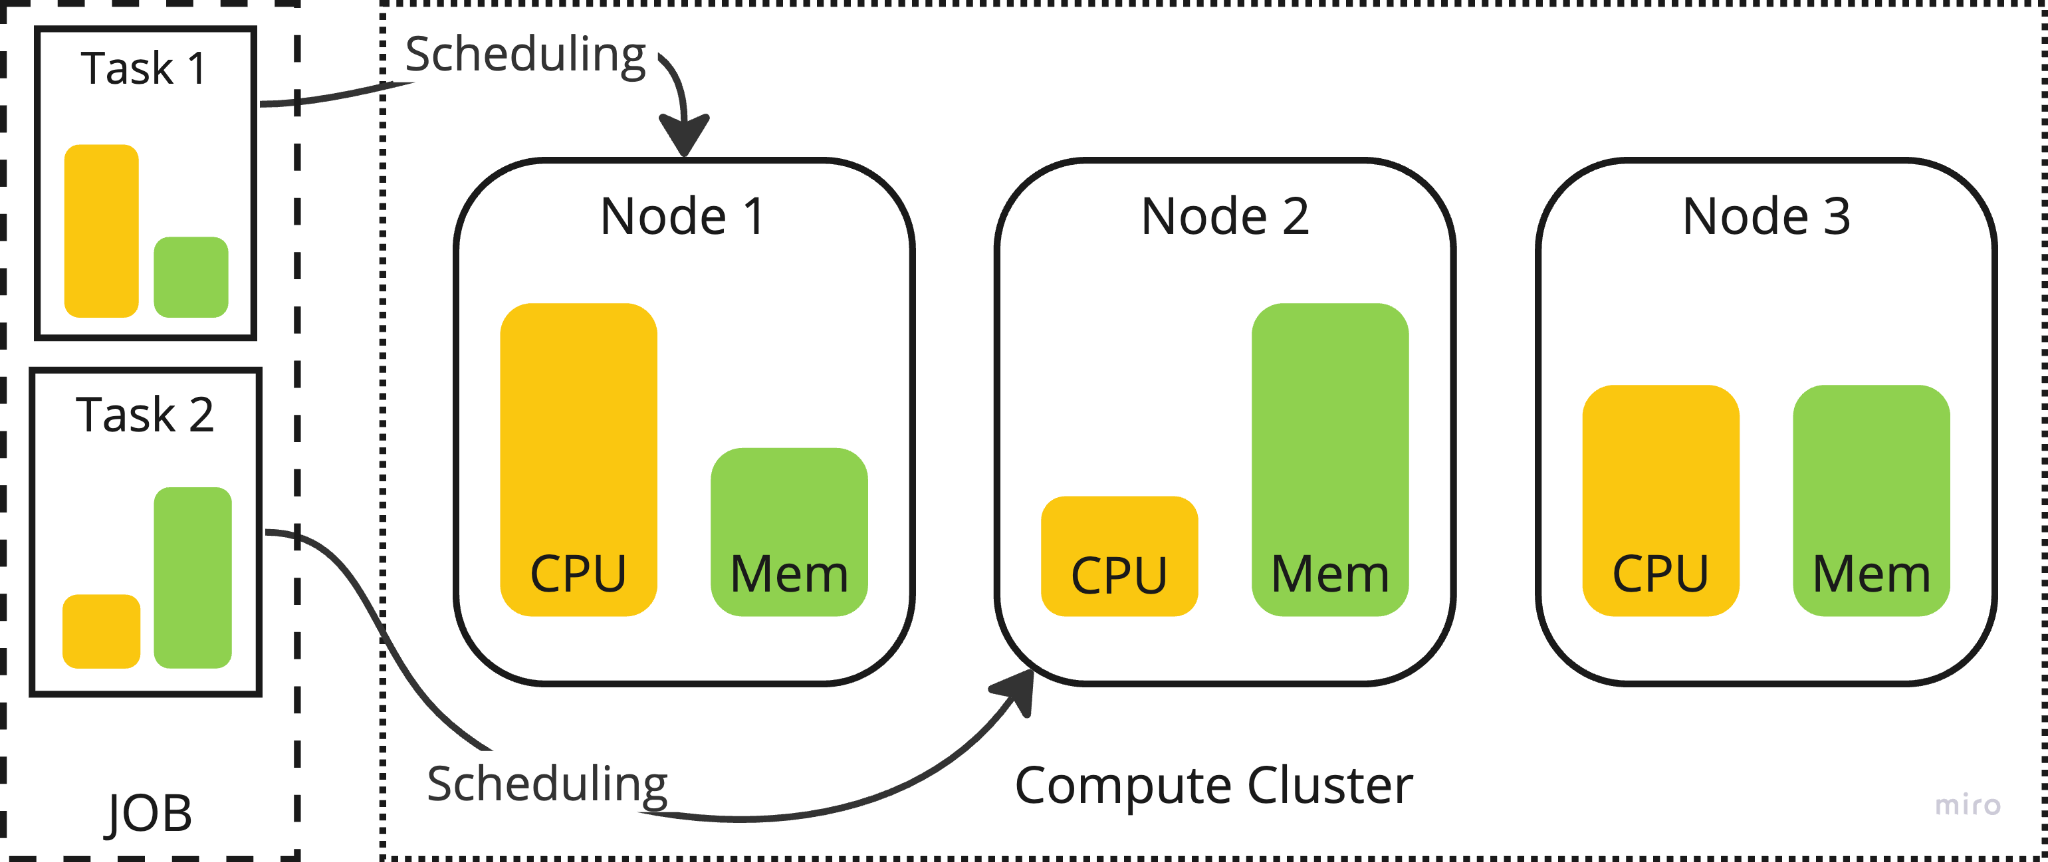
\includegraphics[width=\linewidth]{images/cluster}
			\vspace{0.1cm}
			\caption*{Simple model of cluster architecture}
		\end{figure}


	\end{frame}

	\subsection{Two approaches for simulation}

    \begin{frame}[fragile]
    \frametitle{\insertsection} 
	\framesubtitle{\insertsubsection}
	
			\vspace{1cm}
	\begin{columns}[t]
		\begin{column}{0.55\textwidth}
			{\centering \small\texttt{Standard Workload Format (SWF)}}
			\vspace{0.3cm}
			\begin{itemize}
				\item<1-> CPU/memory resources
				\item<2-> Given execution time and resources
				\item<2-> Workload is calculated
				\item<3-> Used in famous cluster traces (e.g. Google traces)

			\end{itemize}
						
		\end{column}
		\begin{column}{0.5\textwidth}
			{\centering  \small\texttt{Custom workloads}}
			\vspace{0.3cm}
			\begin{itemize}
				\item<1-> CPU/memory/disk/network resources
				\item<2-> Given workload and resources
				\item<2-> Execution time is calculated
				\item<3-> NDA
			\end{itemize}
		\end{column}
	\end{columns}


    \end{frame}

	\section{Literature Review}
	\subsection{Existing Simulators}
	\begin{frame}
		\frametitle{\insertsection} 
		\framesubtitle{\insertsubsection}

		\begin{figure}[H]
			\hspace{-1cm}
			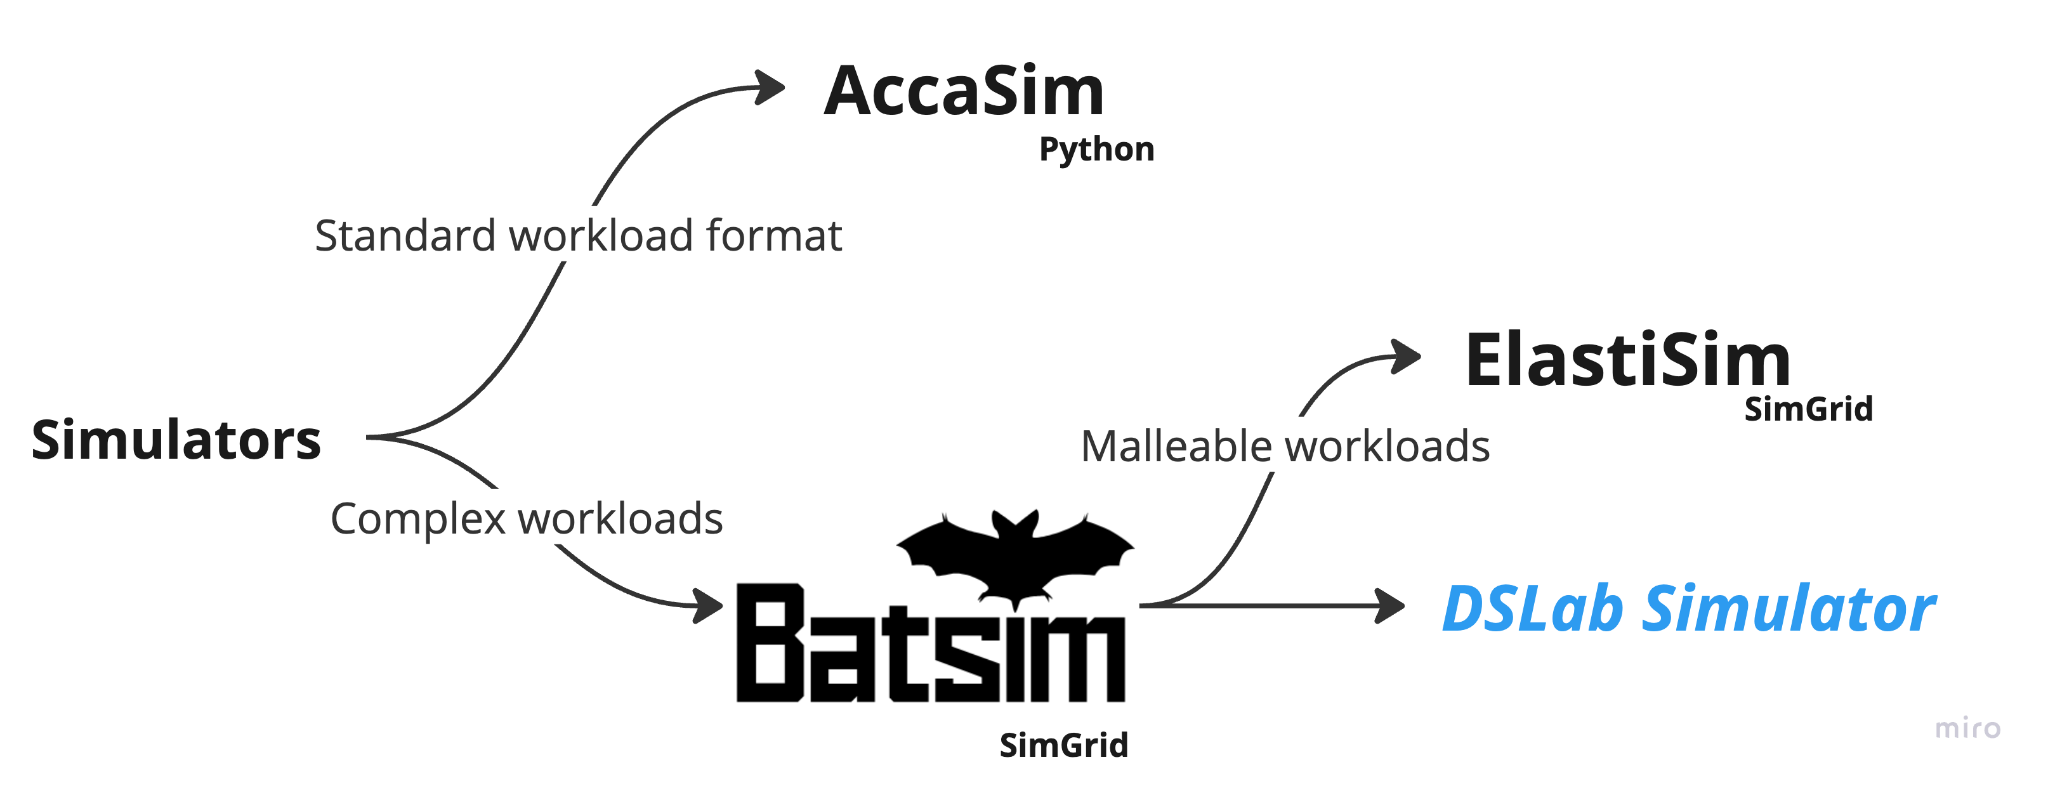
\includegraphics[width=1.1\linewidth]{images/simulators}
			\vspace{0.2cm}
			\caption*{Existing cluster simulators}
		\end{figure}
	\end{frame}

	\subsection{\texttt{BatSim}}

	\begin{frame}[fragile]
		\frametitle{\insertsection} 
		\framesubtitle{\insertsubsection}
		\vspace{1cm}	
		\begin{itemize}
			\item Based on \texttt{SimGrid} simulator platform.
			\item Supports \texttt{SWF} and custom workloads defined as JSON profile.
			\item Supports connecting scheduling algorithms using inter-process communication.
		\end{itemize}
		\end{frame}

	\subsection{\texttt{BatSim Workload format}}
	\begin{frame}[fragile]
		\frametitle{\insertsection} 
		\framesubtitle{\insertsubsection}
		\begin{figure}
			\scriptsize
		\begin{jsoncode}
"jobs": [
  {"id": "job1",  ...  "res": 4, "profile": "sequence"},
],

"profiles": {
  "homogeneous": {
    "type": "parallel_homogeneous",
    "cpu": 10e6,
    "com": 1e6
  },
  "sequence": {
    "type": "composed",
    "repeat" : 4,
    "seq": ["simple","homogeneous","simple"]
  },
}
		\end{jsoncode}
	\end{figure}
	\end{frame}


	\section{Methods}
	\subsection{\texttt{DSLab}}


	\begin{frame}
		\frametitle{\insertsection} 
		\framesubtitle{\insertsubsection}


		\begin{multicols}{2}
			\begin{itemize}
			\item Fast \& scalable simulation platform  
			\item Written in Rust 
			\item Provides models of compute/network/storage  
			\end{itemize}
		\end{multicols}
		
		\begin{figure}[H]
			\centering
			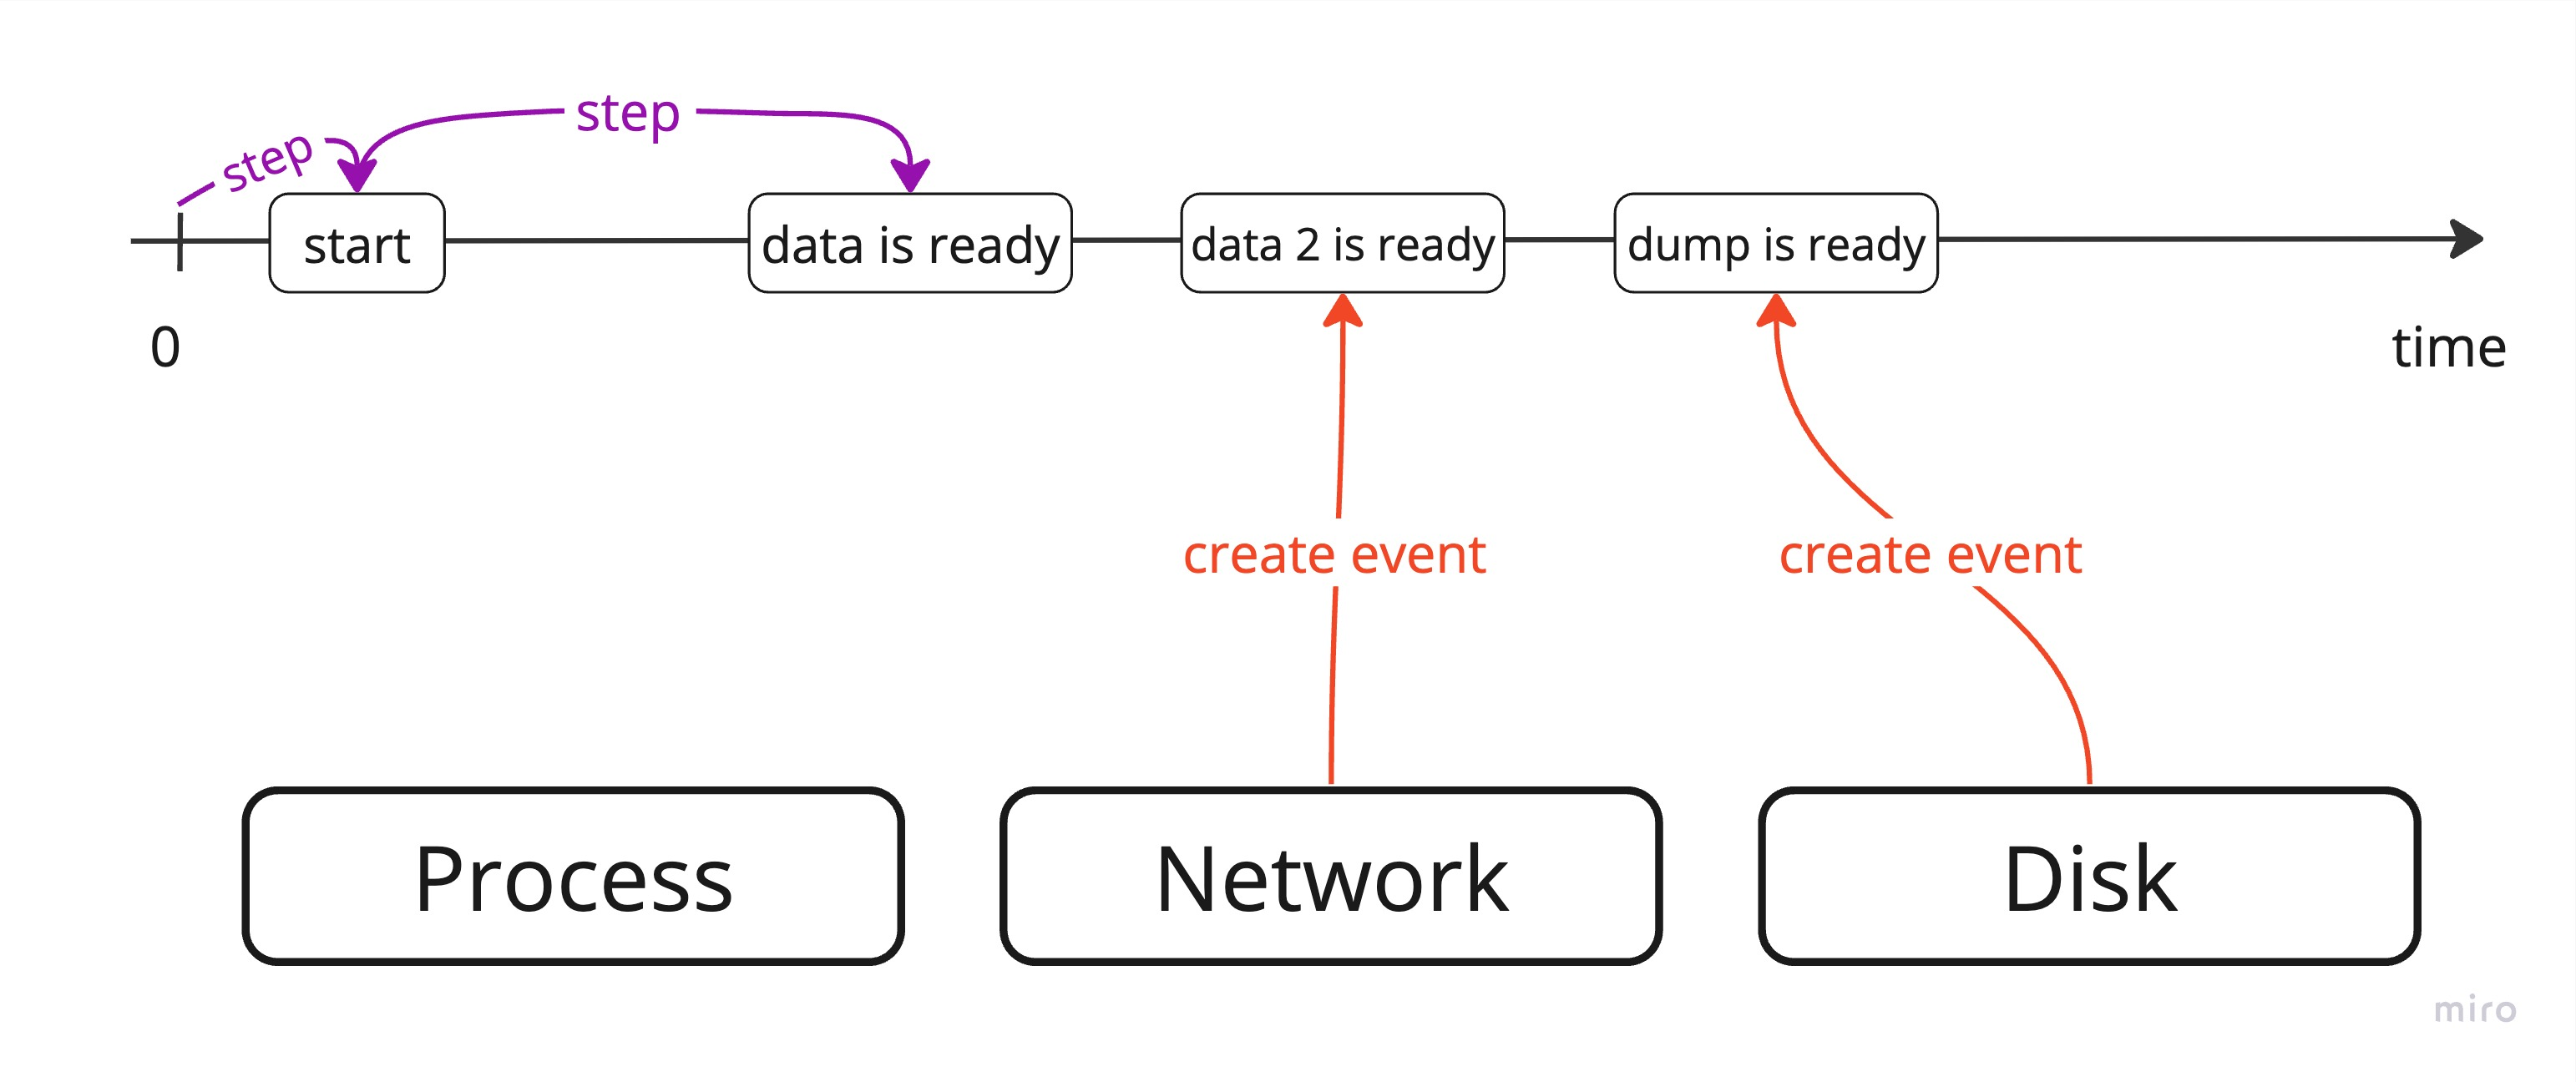
\includegraphics[width=\linewidth]{images/event_pipeline_6}
			\caption*{Discrete-event modeling in \texttt{DSLab}}
		\end{figure}
		
	\end{frame}

	\subsection{Asynchronous event management. Rust futures combiners}


	\begin{frame}[fragile]
		\frametitle{\insertsection} 
		\framesubtitle{\insertsubsection}
		\begin{columns}[t]
			\begin{column}{0.6\linewidth}
			\begin{figure}
				\centering
				\scriptsize

				\begin{rustcode}
async fn process_task(&self, req: TaskRequest) {
  let mut task = TaskInfo {req};

  self.download_data(&task).await;
  self.read_data(&task).await;
  self.run_task(&task).await;
  self.write_data(&task).await;
  self.upload_result(&task).await;
}
				\end{rustcode}

				\caption*{Example of sequent task execution}

			\end{figure}
		\end{column}

		\begin{column}{0.6\linewidth}
\begin{figure}[H]
    \scriptsize
\begin{rustcode}
async fn run(&self, args: JobArgs) {    
  futures::join!(
    self.download_data(args.node_1),
    self.download_data(args.node_2),       
  )
}
\end{rustcode}
\vspace{1.3cm}
\caption*{Example of parallel tasks execution}
\end{figure}	
		\end{column}
		\end{columns}
	\end{frame}

\subsection{JobProfile trait}

	\begin{frame}[fragile]
		\frametitle{\insertsection} 
		\framesubtitle{\insertsubsection}
		
		\vspace{1.5cm}
\begin{figure}[H]
    \small
\vspace{-0.4cm}    
\begin{rustcode}
pub trait JobProfile {
  async fn run(self: Box<Self>, ctx: JobContext)
}
\end{rustcode}
\caption*{Job trait description}
\end{figure}

	\end{frame}

	\subsection{Simulator architecture}

	\begin{frame}[fragile]
		\frametitle{\insertsection} 
		\framesubtitle{\insertsubsection}
		
		\vspace{0.5cm}
\begin{figure}[H]
	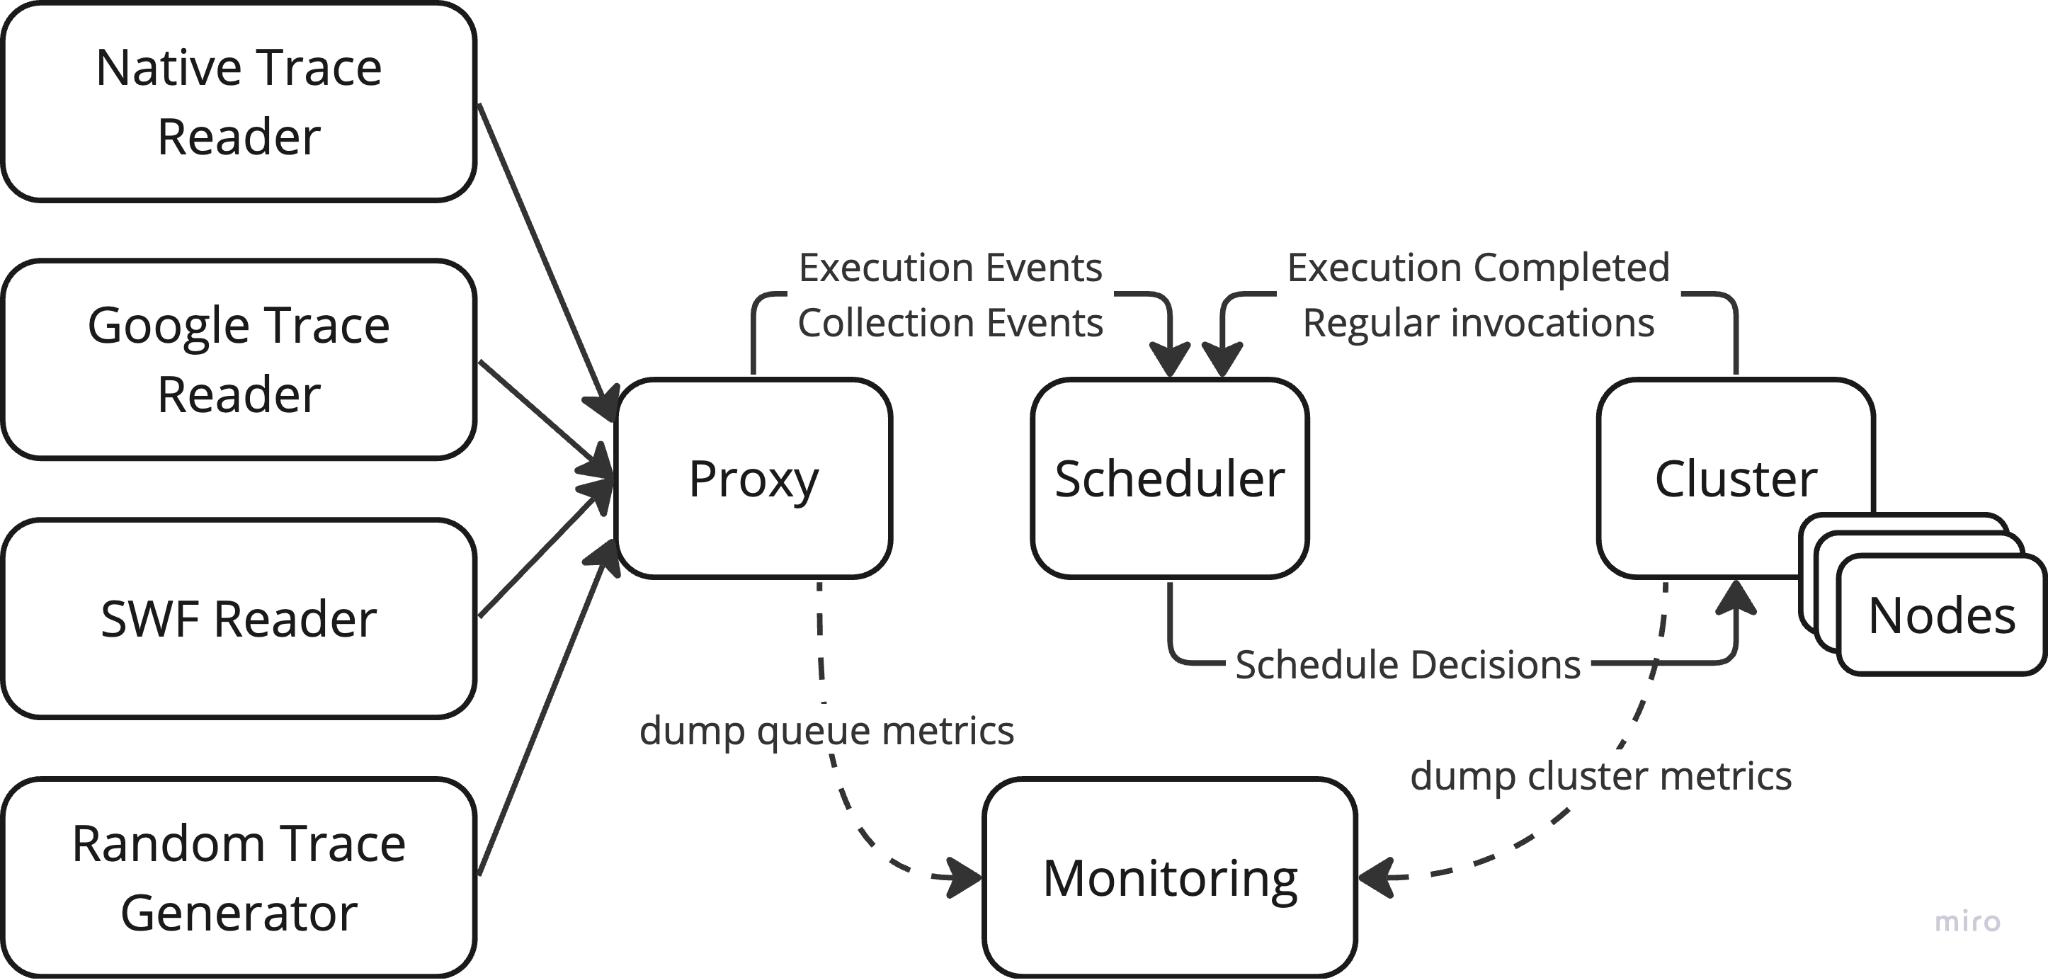
\includegraphics[width=\linewidth]{images/simulator_arc}
	\caption*{Simulator architecture}
\end{figure}

	\end{frame}

	\section{Expected Results}
	\subsection{Fast and scalable compute cluster simulator}
	\begin{frame}[fragile]
		\frametitle{\insertsection} 
		\framesubtitle{\insertsubsection}
		\vspace{1cm}
		\begin{itemize}
			\item[\ding{51}] \texttt{SWF}-based simulation 
			\item Custom workload simulation
			\item Support reading workload traces from popular sources (Google, Alibaba)
			\item Support for collecting metrics during the simulation and writing them to a file with the results
			\item High performance, support for cluster modeling from 1-10K servers
		\end{itemize}

	\end{frame}

	\section{References}
	\begin{frame}
		\frametitle{\insertsection} 
		\framesubtitle{\insertsubsection}
		\vspace{1cm}	
		\begin{enumerate}
			\item The standard workload format specification. \url{https://www.cs.huji.ac.il/labs/parallel/workload/swf.html}
			\item Dslab repository. \url{https://github.com/osukhoroslov/dslab}
			\item BatSim docs. \url{https://batsim.readthedocs.io/en/latest/}
		\end{enumerate}
		% \printbibliography
	\end{frame}

\end{document}